\documentclass[a4paper,12pt]{article}
\usepackage{polski}
\usepackage[utf8]{inputenc}
\usepackage{graphicx}
\author{Marcin fabrykowski}
\title{Dźwięk i muzyka. Lab 09. Modulacja AM i FM}
\begin{document}
\maketitle
\newpage
\section{Modulacja AM}
Naszym zadaniem jest zaprojektowanie modulatora AM. Przykład takiego modulatora widać na rys.~\ref{fig:AM}
\begin{figure}[h]
\hspace{-2.5cm}
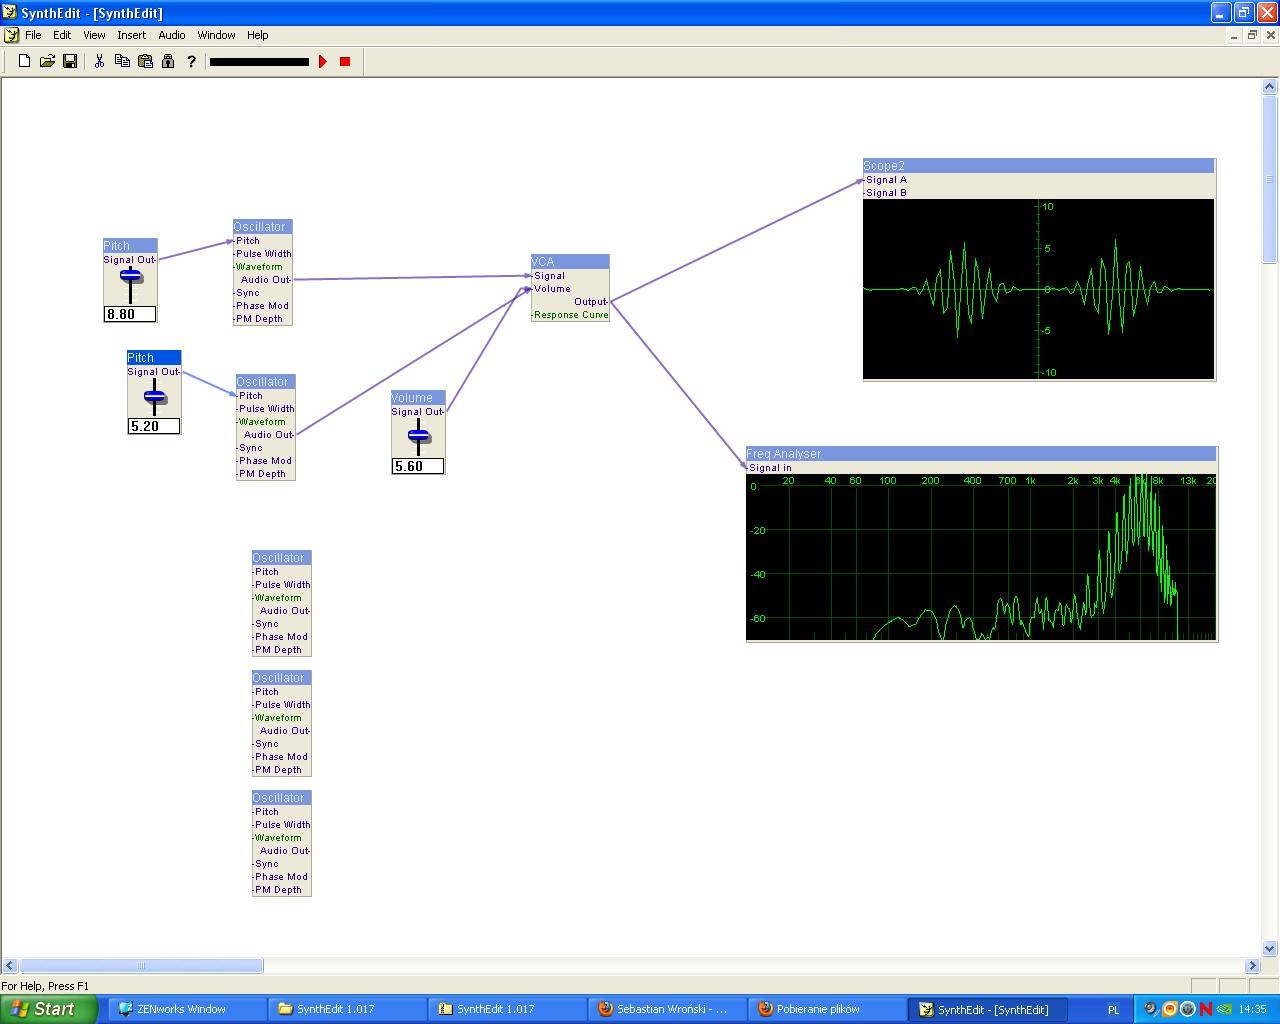
\includegraphics[scale=0.4]{1.PNG}
\caption{Syntezator AM}
\label{fig:AM}
\end{figure}
\section{Modulacja FM}
Naszym zadaniem jest zaprojektowanie modulatora FM. Przykład takiego modulatora dla różnych parametrów widać na rys: \ref{fig:FM1},\ref{fig:FM2},\ref{fig:FM3}

\begin{figure}[h]
\hspace{-2.5cm}
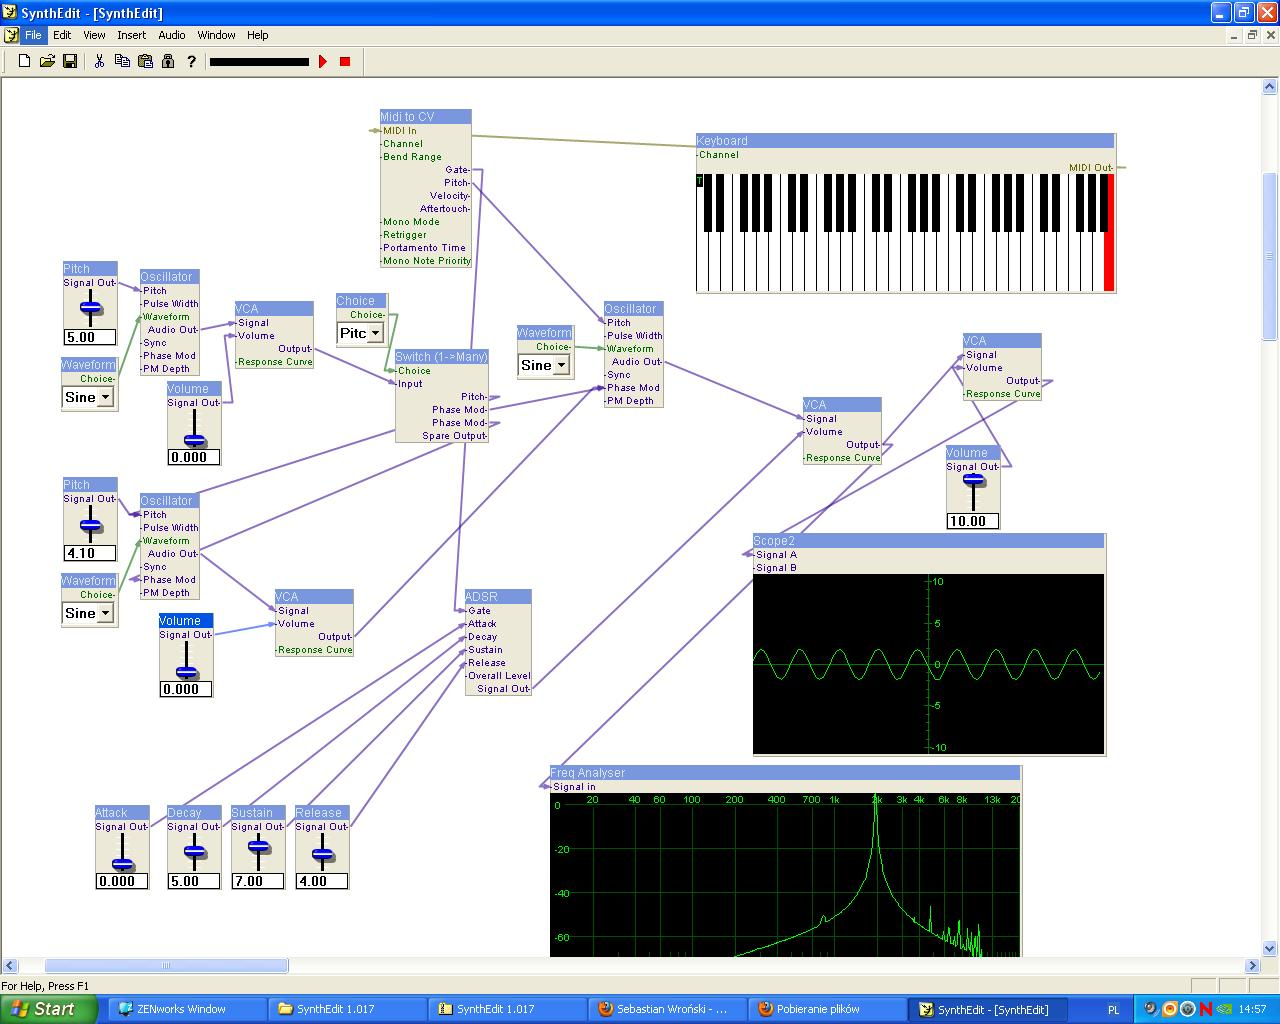
\includegraphics[scale=0.4]{2-01.PNG}
\caption{Syntezator FM}
\label{fig:FM1}
\end{figure}
\begin{figure}[h]
\hspace{-2.5cm}
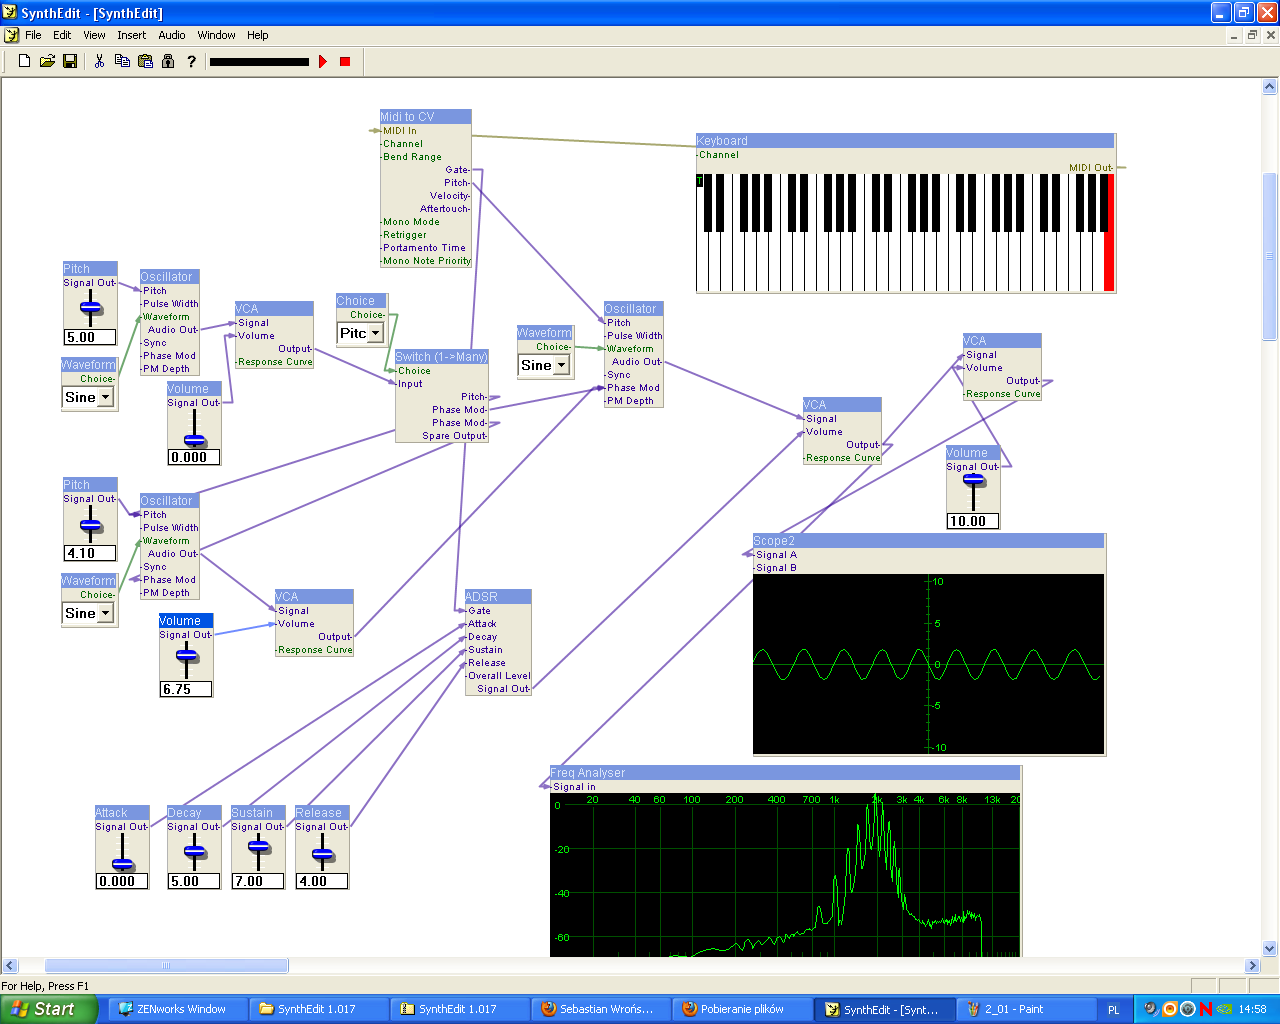
\includegraphics[scale=0.4]{2-02.PNG}
\caption{Syntezator FM, cd}
\label{fig:FM2}
\end{figure}
\begin{figure}[h]
\hspace{-2.5cm}
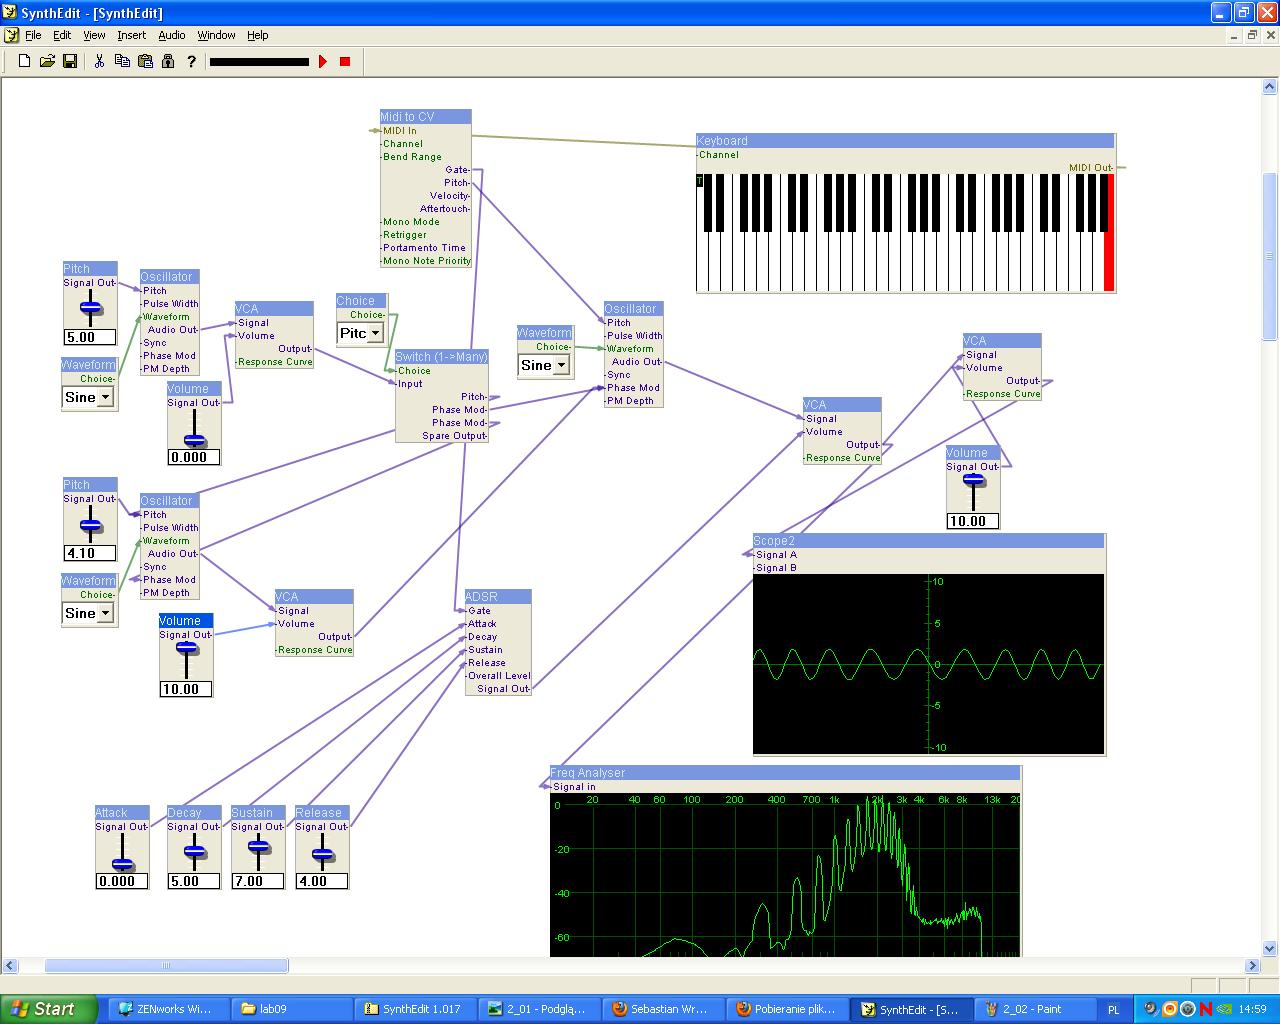
\includegraphics[scale=0.4]{2-03.PNG}
\caption{Syntezator FM, cd}
\label{fig:FM3}
\end{figure}
\end{document}
